\documentclass[onecolumn, draftclsnofoot, 10pt, compsoc]{IEEEtran}

\usepackage{graphicx}                                        
\usepackage{float}
\usepackage{color}
\usepackage{url}
\usepackage{balance}
\usepackage[TABBOTCAP, tight]{subfigure}
\usepackage{enumitem}
\usepackage{pstricks, pst-node}
\usepackage[T1]{fontenc}
\usepackage[font=footnotesize]{caption}
\usepackage{helvet}
\renewcommand{\familydefault}{\sfdefault}

\usepackage{geometry}
\geometry{letterpaper, margin=1in}

\newcommand{\cred}[1]{{\color{red}#1}}
\newcommand{\cblue}[1]{{\color{blue}#1}}
\newcommand{\toc}{\tableofcontents}
\newlength{\drop}

\def\name{Mark Bereza}

\parindent = 0.0 in
\parskip   = 0.1 in

\begin{document}

\begin{titlepage}
\begin{center}

\vspace*{50mm}

\textsc{\LARGE CS472: Computer Architecture}\\[1.5cm]

\hrule
\vspace{5mm}
{ \huge \bfseries UNIVAC 1107 vs ARM11:\\Architecture Comparison\\[0.9cm] }
\hrule 
\vspace{5mm}

\noindent
\begin{minipage}{0.4\textwidth}

\begin{flushleft} \large
\emph{Author:}\\
Mark \textsc{Bereza}
\end{flushleft}
\end{minipage}%
\begin{minipage}{0.4\textwidth}
\begin{flushright} \large
\emph{Instructor:} \\
D. Kevin \textsc{McGrath}
\end{flushright}

\end{minipage}

\vspace*{\fill}
{\large \today}\\
{\large Fall Term}

\end{center}
\end{titlepage}
  
\tableofcontents
\newpage
\renewcommand{\baselinestretch}{1.0}
\linespread{1.0}
\section{Introduction and History}
To gain a better understanding of computer architectures as a whole and how widely different their implementations of certain functionalities can be, this paper will aim to compare the UNIVAC architecture to that of ARM. More specifically, this paper will go over both the UNIVAC 1107's and the ARM11's approaches to instruction set design, datapath design, and memory subsystems before finally discussing how their unique architectural features might boost performance.

Before delving into the technical details of these two vastly different computer architectures, however, it is prudent to first dicuss their history and significance. After all, why should one care about the design decisions employed by these seemingly arbitrary technologies? 

We will begin with the more ancient of the two - the UNIVAC 1107, which derives its name from Universal Automatic Computer 1107. The 1100 series began with the UNIVAC 1107, which released in 1962 \cite{univacwiki}. By this time, the brand UNIVAC has already made a name for itself by releasing the first commercially available computer in the United States, the UNIVAC I, in 1951. By the time Remington Rand (by then it had become Sperry Rand) released the UNIVAC 1107 11 years later, huge improvements had been made to the design since its fore-running ancestor first hit the market. Many of the fundamental features of modern computers were not made available on UNIVAC machines until the release of the 1107, which is why it and not the UNIVAC I was chosen for this comparison. Some of the bold new features (at the time) included solid state memory, the EXEC I and EXEC II operating systems, a Fortran compiler, and its own assembly language named SLEUTH. Despite these improvements, the 1107 is still the size of a room and extremely expensive. In fact, a standard configuration would cost about \$1.6 million in 1968, and that's not accounting for inflation \cite{univacprice}. Suffice it to say, the UNIVAC 1107 is still very far from being a "personal computer". Instead, these machines were purchased by large companies and universities and a single machine's computation power would be shared among many users. Looked at another way, the simple fact that organizations were willing to pay such a premium for the UNIVAC is indicative of how valuable its computation power was in the 1960s.

The ARM architecture, originally an abbreviation of Acorn RISC Machine, did not release its first product until 1985, over 20 years after the release of the UNIVAC 1107 \cite{armwiki}. The first ARM chips were vastly different from the ones one might find in Raspberry Pis or smartphones today; they were created to function as extremely simple coprocessors for other architectures. The RISC in Advanced RISC Machine refers to Reduced Instruction Set Computing, a strategy where a processor's instruction set is kept extremely basic in order to reduce the average number of cycles needed per instruction. Despite drastic changes in ARM's technology over the years and its rebranding in 1990, ARM chips continue to follow the RISC strategy. Today, ARM is famous for controlling over 90\% of the embedded systems market and residing in over 95\% of the world's smartphones \cite{armslides} \cite{armwiki}. In raw terms, over two billion ARM processors are shipped each year \cite{armslides}. Of the numerous ARM architectures, the ARM11 was chosen primarily because it is well-documented and it is the only model released using the ARMv6 architecture, making the ARM11 chip somewhat synonymous with that architecture as a whole. 
\section{Instruction Set Design}
\subsection{ARM11}
One of the most fundamental aspects of any computer architecture is how its set of machine instructions is designed. In fact, ARM decided that its instruction set strategy, RISC, is so integral to its identity that they stuck it right in the name. The ARM11 actually utilizes a combination of two instruction sets: the 32-bit ARMv6 ISA and the 16-bit Thumb ISA \cite{armslides}. This is accomplished by allowing ARM systems to operate in two distinct states: the ARM state and the Thumb state. 

The ARM instruction set, as of ARMv6, contains 148 unique instructions split into the following categories, based on the type of operation \cite{armreference}:
\begin{enumerate}
\item \textit{Branch instructions} allow the processor to jump up to 32 MB forward or backward in the currently executing program based on some condition. The Branch with Link instruction also allows for the existence of subroutine calls by saving the address of the instruction right after it (the return address) before performing the jump.
\item \textit{Data-processing instructions} are the superset of basic addition/subtraction operations, basic logical operations (AND/OR), comparison operations, and move operations. All but the move operations take two operands as input, one of which must be a register. The other may be either a register or some intermediate value. 
\item \textit{Multiply instructions}, as the name would suggest, are instructions which facilitate multiplication of two values. Since multiplication of two $n$-bit values requires up to $2n$-bits to store the result, the multiplication instructions provided come in a variety of flavors based on how the result is calculated and stored, including a normal multiply that stores the lower 32-bits, a long word multiply that stores the entire 64-bit result across two registers, halfword multiplies, most significant word multiplies, and more.
\item \textit{Parallel addition and subtraction instructions}, new to ARMv6, perform addition and/or subtraction operations in parallel on either halfwords or bytes.
\item \textit{Extend instructions}, also new to ARMv6, allow bytes or halfwords to be extended, zero extended, or sign extended to halfwords or words.
\item \textit{Status register access instructions}, as the name would imply, allow the user to move the contents of the status register.
\item \textit{Load and store instructions} allow the bytes, halfwords, or one or more words to be moved between registers and memory. ARMv6 provides many load and store instructions, each varying based on the addressing-mode, signed vs. unsigned, size of the operation, and more.
\item \textit{Semaphore instructions} perform load and store operations atomically and are vital in the construction of synchronization constructs, hence the name.
\item \textit{Exception-generating instructions} facilitate software interrupts and software breakpoints by forcing certain exceptions to be thrown.
\item \textit{Coprocessor instructions} facilitate communication between an ARM processor and its coprocessor.
\item \textit{Other miscellaneous instructions} is a catch-all category for instructions that don't fit neatly into any of the other categories. These including lead-zero counting, byte order reversal, saturation, and others.
\end{enumerate}
Beyond these existing instructions, the ARM ISA also provides extension space so that additional instructions may be added in future versions in a logical fashion. 

If one was to try and perform some synthesis based on the ARMv6 ISA's list of instructions, one might accurately conclude that ARMv6 is a product of a long, iterative development history. The numerous seemingly arcane or corner-case instructions are a result of the ISA adapting and expanding to improve the performance of common real world tasks in a heuristic manner. Instead of operating systems and higher level programming languages growing naturally out of a short list of fundamental operations, the design behind these supposedly fundamental operations is bent to accommodate high level system constructs like semaphores and software breakpoints. Overall, it seems that the instruction set was designed with performance as a priority, which makes sense when ones considers that ARM runs primarily on small embedded systems featuring limited hardware.

As for the encoding of instructions into 32-bit words, the format varies significantly based on the type of instruction, but some common patterns can be found. Firstly, almost every ARMv6 instruction can be executed conditionally based on the state of certain flags in the control register. For such instructions, bits 31:28 are used to encode the condition. Bits 27:24, on the other hand, are often used to specify the category of the instruction, thereby controlling how the remaining bits are interpreted by the system. Bits 24:20 are often used to encode the specific opcode for the instruction and occasionally some control flags. For instructions that take two arguments, bits 19:16 are often used to encode the register number of the first operand (source) and bits 15:12 are used to encode the register number of the second operand (destination). The remaining bits are the most likely to vary based on the instruction type and may be used for anything from immediate memory addresses to offsets to shift values. It is apparent that ARM is more than willing to trade off simplicity of instruction format for space efficiency because allowing the format to change based on the instruction type allows a large number of fairly sophisticated instructions to be encoded in just 32 bits. This further proves that the ARMv6 ISA prioritizes memory efficiency and performance.

The rationale behind including the 16-bit Thumb instructions, on the other hand, lies with the fact that the ARM architecture is often used in very small embedded systems featuring minimal memory. By consuming an additional processor cycle, the 16-bit Thumb instructions are converted into their ARM counterparts during runtime. The reason why this conversion can occur in a single cycle is because the Thumb ISA is "a re-encoded subset of the ARM instruction set" \cite{armreference}. Moreover, Thumb instructions are performed on the same architecture model (32-bit values, 32-bit addresses) as the regular ARM instructions, just with limited functionality. To help accommodate the short instruction length, Thumb instructions only have access to the first eight general purpose registers. Here, the ARM architecture trades simplicity not for performance but rather portability across a wide array of hardware.
\subsection{UNIVAC 1107}
Unsurprisingly, the instruction set design for the UNIVAC 1107 is vastly different. Unlike ARM, which uses a combination of 32-bit word and 16-bit halfword instructions, all instructions for the UNIVAC are the size of a single 36-bit word \cite{univacarch}. These instructions can then operate on data of sizes ranging from a field within a word to multiple words, similar to ARM instructions. Figure 1 shows the various data formats supported by the UNIVAC 1107's ISA.\\ \\
\begin{minipage}{\linewidth}
\begin{center}
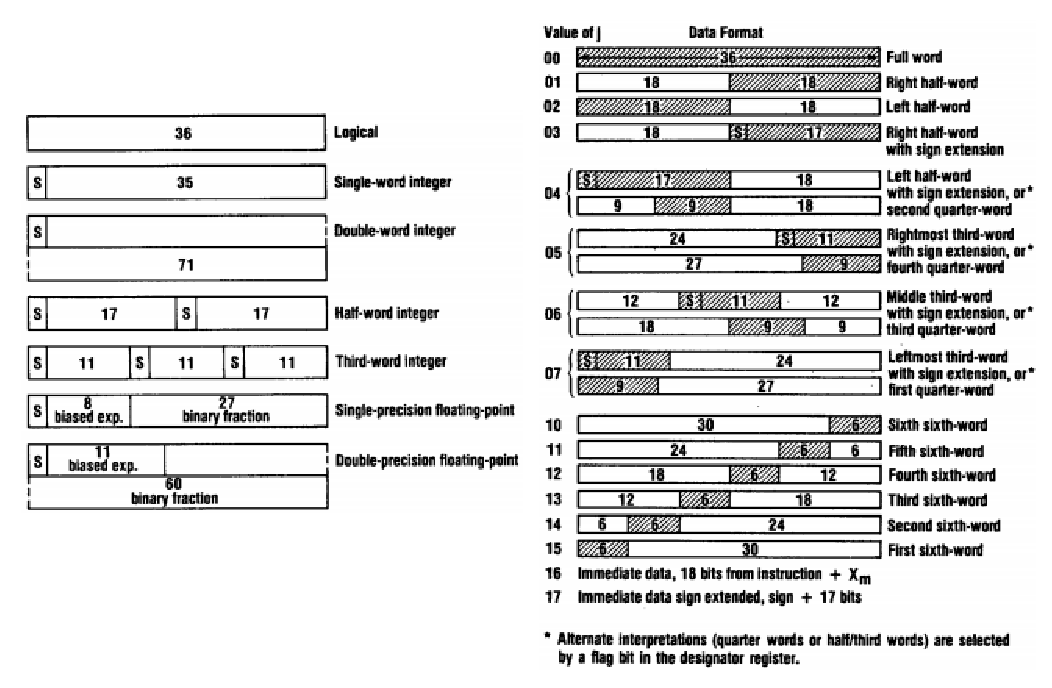
\includegraphics[width=\textwidth]{figure1.eps}
\captionof{figure}{The data formats (logical, arithmetic, and partial word size) supported by the UNIVAC 1107's ISA \cite{univacarch}}
\end{center}
\end{minipage}
\\ \\ Although UNIVAC 1107 can select partial words in its operation code, the minimum addressable unit of memory is a single 36-bit word, far worse than the byte-addressable ARM11 architecture. 

The UNIVAC 1107's SLEUTH II assembly language (later renamed to just "assembler") contains 117 unique instructions. As for the functionality provided by these instructions, SLEUTH II naturally lacks instructions to facilitate modern operating system features like semaphores and software breakpoints, but does provide sophisticated logical and arithmetic operations not found on ARMv6 like floating point operations (although these are made available to ARM11 via a floating point coprocessor), division, parity testing, XOR, and searches (both masked and unmasked). Moreover, SLEUTH II lacks many of the edge-case specific operations made available in ARMv6. What can be concluded from all this? Well, first off, it is clear that unlike ARMv6, the SLEUTH II ISA is designed with human usability in mind and not hardware performance. The intuitive and general-purpose nature of each of its instructions conveys the idea that SLEUTH II is something its designers intended for programmers to write directly, which makes sense since the majority of code at the time was still written in assembly and it has been less than a decade since the invention of the first compiler \cite{compilers}.

Additionally, unlike ARM11, the UNIVAC 1107 implements CISC, not RISC. This can be concluded because its instructions obtain one operand from registers and the other from memory, a telltale sign of a CISC architecture. Because CISC requires fewer instructions to accomplish the same functionality, it is inherently more memory-efficient than RISC. In light of this, it makes sense for system like UNIVAC 1107, created when memory was a very expensive luxury, to utilize CISC. Additionally, utilizing CISC allows UNIVAC to perform operations directly on memory locations, whereas ARM is forced to move data into registers before it can manipulate them.

SLEUTH II also differentiates itself from ARM and most other modern ISAs by following the same instruction encoding format for every one of its instructions. More specifically, each of its instructions is subdivided into fixed-size, fixed-order fields:
\begin{enumerate}
\item The first field, \textit{f}, is 6 bits wide and holds the major function code.
\item The second field, \textit{j}, is 4 bits wide and holds the minor function code.
\item The third field, \textit{a}, is 4 bits wide and is used to specify an operand register.
\item The fourth field, \textit{x}, is 4 bits wide is used to specify an index register.
\item The fifth field, \textit{h}, is a single bit flag that indicates index incrementation.
\item The sixth field, \textit{i}, is a single bit flag that indicates indirect addressing.
\item The seventh field, \textit{u}, is 16 bits wide and holds either an address offset or the address of an immediate operand.
\end{enumerate}
The decision to make instructions follow a strict format is likely motivated by two factors: (1) it keeps the instruction set simple for developers who still coded directly in assembly and (2) because implementing the sophisticated hardware necessary to change how instructions are decoded based on the opcode was simply not feasible with the technology available at the time.

One final major way that UNIVAC 1107 instructions differ from those of ARM11 is that negative values are stored in one's complement and not two's complement. Since the two's complement representation of negative values avoids the issue of "negative zero" inherent to one's complement and allows for arithmetic operations to be performed the same way on values regardless of sign, it's difficult to understand why older systems like UNIVAC used one's complement besides "it is a lesson learned over time". Another possibility is that one's complement ensures that negation will never fail since it simply flips all the bits.
\section{Datapath Design}
\subsection{ARM11}
Another fundamental aspect of any computer architecture is the design of the datapath - the path data takes through the system's various hardware components as instructions are fetched and executed. The ARM11 utilizes an eight stage pipeline. Pipelines serve to segment instructions into tasks that can be performed concurrently, thus allowing instructions to be retired in the time it takes to complete a single stage of the pipeline as long as said pipeline remains full. Longer pipelines often mean shorter time needed to complete a single stage and thus result in higher best-case performance. On the other hand, longer pipelines require high clock speeds to drive, which can consume significantly more power and produce significantly more heat, highly undesirable traits for the low-power embedded systems ARM tends to run on. Additionally, longer pipelines take longer to fill and thus take longer to reach peak performance and as a consequence are more vulnerable to branching code that constantly clears the pipeline. In this way, pipeline depth is a tight balancing act between performance, power consumption, and branch handling. Since embedded systems do not require the raw performance expected of desktop CPUs and since power consumption is a more apparent limiting factor for them, the ARM11 architecture shies away from Intel-sized (14 stage) pipelines. On the other hand, ARM11 has a deeper pipeline than previous versions of the ARM architecture, which only had three or five stages. This is because ARM11 features branch prediction, which helps to mitigate some of the risk of the pipeline being emptied at every branch. It is also because the ARMv6 ISA running on the ARM11 allows for more sophisticated instructions, like longword multiplication, which are difficult to implement in fewer stages. Interestingly, the process of branch prediction itself complicates instructions and resulted in a second fetch stage being added to the pipeline specifically to perform branch prediction. Figure 2 illustrates each of ARM11's eight pipeline stages and matches each to which hardware components it touches within the datapath.\\ \\
\begin{minipage}{\linewidth}
\begin{center}
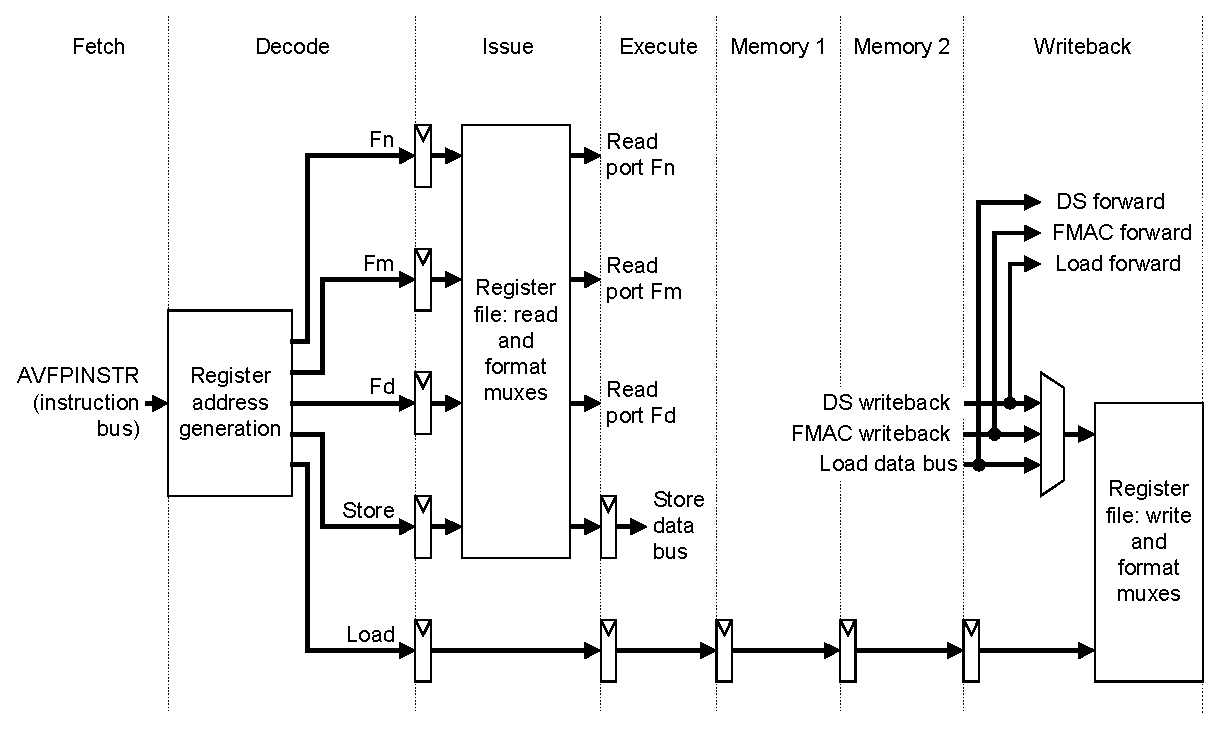
\includegraphics[width=\textwidth]{ls_pipeline.eps}
\captionof{figure}{The ARM11 pipeline stages \cite{armpipeline}}
\end{center}
\end{minipage}
\\ \\ In the first two stages, the next instruction is fetched by moving it from the instruction bus to the register address generation block. It is also during these two stages that branch prediction is performed. Two different strategies are employed by ARM11 in order to predict the likely outcome of code branches. The first, called the dynamic branch predictor, maintains a record of which branches have already been seen and which branches have been taken the most or least often \cite{arm11micro}. The processor then uses this historical information to make a best guess at what branch will be taken. In the case where no historical record is available for an encountered branch, the second strategy, static branch prediction, is used \cite{arm11micro}. In static branch prediction, the processor takes branches that jump backwards in program memory (presuming that these branches are loops) and doesn't take branches that jump forwards in program memory. 

In the third stage, the instruction is decoded and routed to the appropriate registers in the register file. In the fourth stage, the pertinent registers are read and the instruction is issued. From here, the stages change depending on the instruction being executed. In the standard ALU path, the final four stages are: (1) perform any required shifting on the second operand before passing it to the ALU, (2) perform the ALU operation, (3) saturate the result, and (4) write the result back to the register file. In the multiplier path, three of the four stages are simply segments of a single multiplication operation and the final stage writes the result back to the register file as before. Finally, in the load/store path, the final four stages are: (1) data address calculation is done by the ALU, (2) and (3) involve accessing the data cache, and (4) data is written back to the Load Store Unit (LSU).

Utilizing different data paths for memory access and arithmetic/logic operations has the added benefit of allowing for some inter-instruction parallelism when both functionalities are required by a single operation \cite{armslides}. Moreover, this separation allows for one path to continue executing even if the other encounters a delay resulting from a cache miss. As before, it is clear that the biggest driving force behind the ARM architecture is performance.

As for the registers available to ARM11, they include 16 general-purpose registers, 17 mode-specific registers used for things like exception handling, and 7 status registers \cite{armslides}.

\subsection{UNIVAC 1107}
Like the ARM11, the UNIVAC 1107 is also a multi-cycle system. Unlike the ARM11, however, it did not implement instruction pipelining. This is likely because pipelining muddies up assembly coding because the developer can no longer presume that each instruction completes before the next one is fetched. For ARM11, an architecture designed in an era where high level languages hide such messy details from the developer, this is a non-issue. In the days of the UNIVAC, though, invalidating sequential execution was a big deal.

According to \textit{The Architecture of the Sperry UNIVAC 1100 Series Systems}, instruction execution would occur via the following steps:
\begin{enumerate}
\item The instruction would be first fetched and decoded.
\item Next, the address of the storage operand would be calculated.
\item Then, register and storage operands would be fetched, in that order.
\item After that, the now fetched storage operand would be reformatted.
\item Then, the actual operation would be performed on the acquired operands.
\item Finally, the result would be reformatted and stored.
\end{enumerate}
Slight variations to this data path are also possible. For example, although the default data path for UNIVAC instructions involve one operand obtained from memory and another obtained from the register file, the same instruction could also be performed in a register-register fashion by simply providing the address of a register for the former.

On the subject of registers, it should also be noted that the UNIVAC 1107 has more registers than many modern computer architectures like the ARM11. A total of 128 words of memory is provided via the General Register Set (GSR) \cite{univacarch}. 16 of these are \textit{A} registers, used for arithmetic. 16 of these are \textit{R} registers, used for special control functions. Another 16 (4 overlapping with \textit{A} registers) are \textit{X} registers, used for indexing. Separate copies of these register banks are provided for both user space and the operating system. The remaining registers are special purpose registers used exclusively by the operating system.
\section{Memory Subsystem}
\subsection{ARM11}
ARM11, utilizing 32-bit byte addressing, can address up to 4 GB of physical memory. Although it is common for today's computers and even some smartphones to have more than 4 GB of memory, this was probably sufficient for phones and embedded systems at the time of ARM11's release (2003 to 2005). That being said, the ARM11 does also provide a series of memory access methods that are far from standard. For one, memory words (32-bits) can be indexed using a register and a 12-bit offset and bytes can be indexed using a register and a 8-bit offset \cite{armslides}. Finally, the ARM11 can also perform data transfers in parallel, allowing for up to 16 registers to be moved to/from memory using a single instruction.

ARM11 also supports virtual memory by implementing a Memory Management Unit (MMU) that performs translation between virtual and physical addresses in hardware \cite{arm11manual}. Additionally, the ARM11 implements two layers of Translation Lookaside Buffers (TLBs) to improve the performance of these translations. The first layer queried is called the MicroTLB and it is split into data and instruction sections in a fashion similar to how L1 cache is often segmented. The MicroTLBs are called such because each only holds ten entries. If the MicroTLB misses, the request is passed to the unified main TLB which is slower but also larger, holding up to 64 entries. If the main TLB also misses, a page table walk is performed.

As for caching, two levels are available on the ARM11 architecture. The first level consists of data and instruction L1 caches, data and instruction Tightly-Coupled Memory (TCM) areas, and a write buffer \cite{arm11manual}. The L1 cache is four-way set associative and can range in size from 4 KB to 64 KB. The TCM provides high speed memory similar to cache, but without a lot of the unpredictability, making it useful for storing data structures lacking in locality. These TCMs can range in size from 0 KB to 64 KB. Finally, the write buffer, as the name might suggest, is simply a buffer that holds queued memory writes. The second level of caching provides an interface for L2 caching per the ARMv6 standard but no L2 cache is present on ARM11 chips by default.
\subsection{UNIVAC 1107}
Despite having a larger word size than the ARM11, the UNIVAC 1107 can only address 65,536 words (about 2 MB) of main memory because it uses 16-bit addresses \cite{univacthinfilm}. The short address size is an unfortunate consequence of adhering to a common instruction encoding format for all instructions. Ultimately, however, this proved to be far from a bottleneck for the UNIVAC since this amount of memory alone would cost the modern equivalent of about \$3 million back in 1968 \cite{univacprice}. Perhaps more importantly, the programs being run on the UNIVAC 1107 during its prime were also significantly lighter-weight than the memory-intensive multimedia applications common today.

Unlike the ARM11, the UNIVAC does not implement virtual memory at all. This shouldn't be surprising, though, since the first machine ever to utilize virtual memory was released a few months after the UNIVAC 1107 and the sheer \textit{concept} of virtual memory was only invented a few years before that in 1956 \cite{virtualmemory}. This means that all addressing done on the UNIVAC 1107 references physical memory locations directly. While this is disadvantageous for many reasons, one advantage of not using virtual memory is that one avoids the processing overhead incurred during address translation every time memory is accessed. The trade-off is no contest today but in the 1960s, when transistors were still measured in micrometers and each would cost about \$8 in today's currency, there wasn't much processing power to spare on abstraction layers \cite{transistorprice}.

What's perhaps even more mind-boggling is that the UNIVAC 1107 didn't have any kind of cache; such a feature would not be found in UNIVAC machines until the release of the UNIVAC 1100/80 in 1979, almost 20 years later \cite{univacwiki}. Instead, the UNIVAC 1107 boldly advertised its then-novel thin film solid state register memory, boasting an access time of only 300 nanoseconds \cite{univacthinfilm}. The lack of cache could perhaps also explain why it was designed with a 128-word register file, huge by today's standards.
\section{Conclusion}
Now that we have a basic understanding of these two architectures, it is time to consider how the unique features of each could help boost their performance. 

The ARM11 features a lot of modern computer architecture technologies to help improve performance. For one, by providing the choice between a 32-bit and a 16-bit instruction set, the ARM11 architecture can perform efficiently on a wide array of systems, only using as much memory as necessary. Furthermore, it improves the implementation of complex instructions like floating point and vector operations by including a coprocessor specifically designed to perform these operations in hardware. Beyond that, its relatively deep pipeline and use of branch prediction allows it to retire one instruction per cycle at a high clock rate fairly consistently. Let's also not forget that by isolating cache misses to individual data paths, the performance drop incurred after a cache miss is essentially cut in half. Finally, by providing a two-tier TLB and a TCM in addition to the standard L1 cache, ARM11 boosts performance by providing efficient memory management for edge cases not often considered by other computer architectures.

UNIVAC, on the other hand, being one of the earliest commercial computers, provides very little functionality to boost performance besides its relative large solid state register file. That being said, it could be argued that it achieves better performance not through what it includes but rather through what it doesn't include. For example, by not having the encoding format change based on the opcode of the instruction, less work has to be done during the decoding stage. Additionally, by operating on physical memory instead of virtual memory, the overhead associated with address translation is completely sidestepped.

Overall, it is a wonderful thing that the ARM11 architecture appears to be the clear winner here. It is a testament to how much computer hardware and our understanding of computer architecture has improved over these last 50 years.
\newpage
\bibliographystyle{IEEEtran}
\bibliography{mybib}

\end{document}
